We propose to build an application in which a user can design and test a conveyor belt system. The program hence is a combination of an editor and a simulator. The editor is available in the \textit{building mode}, while the \textit{simulation mode} provides the user a way of testing his or her system. These modes are described in more detail in section \ref{subsec:program-modes}. This project hence has two goals:
\begin{enumerate}
  \item building a user-friendly editor;
  \item implementing nice animations for the simulator.
\end{enumerate}
The program can be used as a game, but could potentially be used as a tool for modelling for example a luggage system at an airport.

\begin{figure}
  \begin{center}
    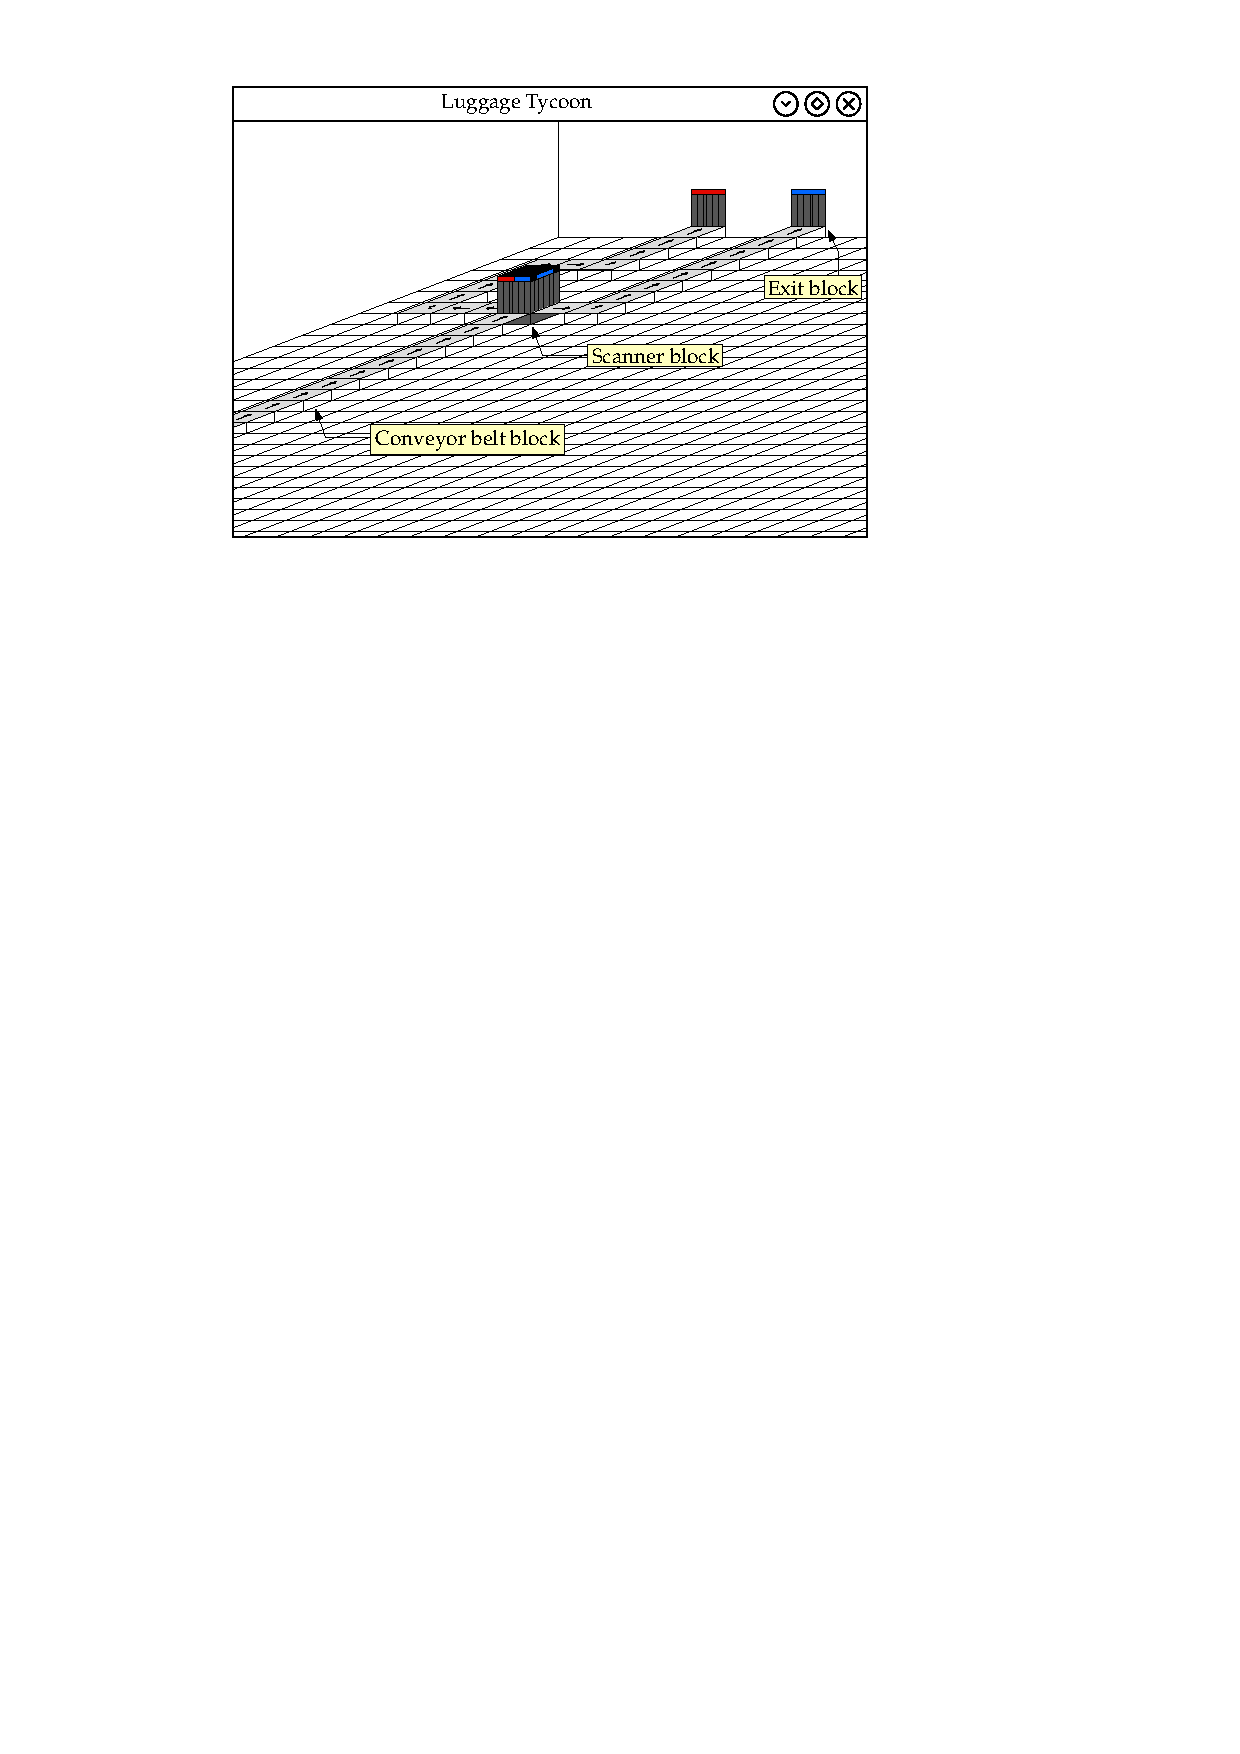
\includegraphics{mockup}
    \caption{A mock-up of the program we want to create.}
    \label{fig:mockup}
  \end{center}
\end{figure}
